\section{Architectural Layers and Elements}
\label{sec:detailed_architecture}

Figure~\ref{fig:detail_ipro} introduces and details the IPro architecture. IPro has four main planes that follow the KDN fundamentals. Next, these plans are detailed.

\begin{figure}[h!]
    \centering
    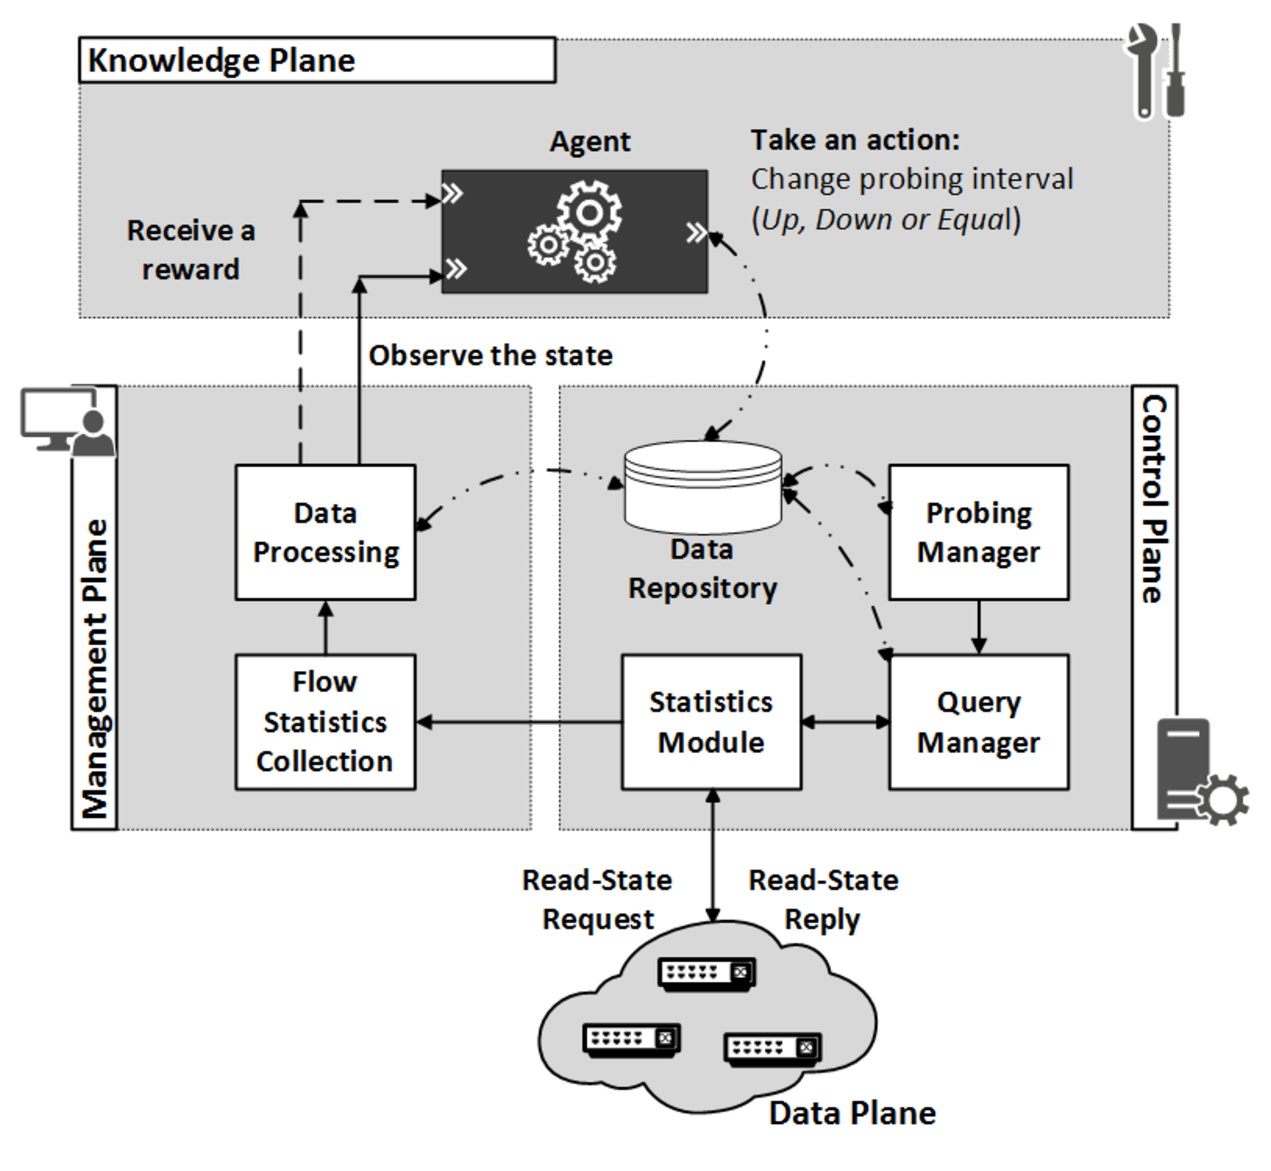
\includegraphics[width=0.60\columnwidth]{figures/Fig2-IPro-architecture}
    \caption{IPro Architecture}
    \label{fig:detail_ipro}
\end{figure}

%\paragraph{\textbf{Knowledge Plane.}}
\subsection{Knowledge Plane}
This plane obtains a rich view and global control over the network from MP and CP. Overall, KP operates in three steps:
\begin{itemize}
    \item It organizes the metadata generated by MP.
    \item It converts that metadata into knowledge by using ML techniques.
    \item It uses that knowledge to make decisions (either automatically or through human intervention) related to routing, traffic classification, anomalies detection, and so on. 
\end{itemize}{}

It is essential to highlight that KP is separated from CP because ML algorithm is generally compute-intensive, and it may affect the performance of CP \cite{mestres_2017:KDN}. In this master dissertation, KP is responsible for learning the network behavior and automatically deciding a new probing interval. KP obtains the current network status and controls the probing interval by interacting with MP and CP, respectively. The KP heart is the RL-agent. This agent is in charge of determining the most-rewarding probing strategy intended to maintain CCO and CUC within target values. IPro considers two thresholds $\omega$ and $\chi$ that are configurable according to network requirements. $\omega$ represents the policy 1 and aims at preventing a high CCO. In turn, $\chi$ represents the policy 2 and aims at preventing a high CUC. To sum up, the RL-agent handles the monitoring policies by controlling $\omega$ and $\chi$. \\

Control policies are defined to prevent monitoring messages from affecting the performance of the controller and the bandwidth of the control channel. For instance, when CUC exceeds 80\% of the CPU capacity, the controller increases its response time, which generates delays and loss \cite{repas_2015:performance_cpu}. In the same sense, when the use of the control channel bandwidth exceeds 80\%, the monitoring messages can interfere with the SDN functions \cite{xu_2017:wildcard_requests}.\\

\begin{figure}[h!]
    \centering
    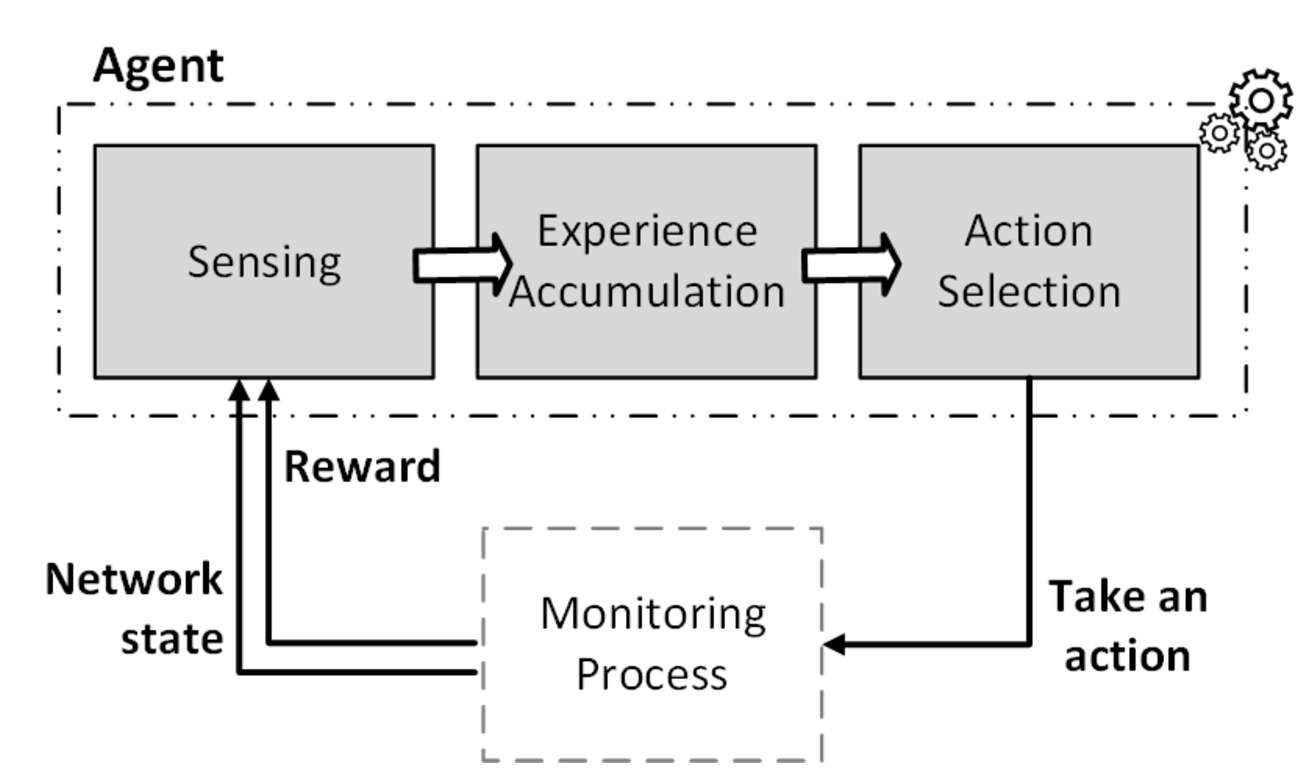
\includegraphics[width=0.50\columnwidth]{figures/Fig3-IPro-agent}
    \caption{The RL-agent General Model}
    \label{fig:ipro_agent}
\end{figure}

Figure~\ref{fig:ipro_agent} depicts the general model of the RL-agent. This model includes three elements, namely, \textit{Sensing}, \textit{Experience Accumulation}, and \textit{Action Selection}. \textit{Sensing} enables the RL-agent to get the network state and the reward of the IPro monitoring process. The \textit{Experience Accumulation} element guides the policy (i.e., what action to take) of the agent in two steps. In the first one, this element combines the observations made by \textit{Sensing} and defines the information matrix that represents the internal states of the RL-agent. In the second step, \textit{Experience Accumulation} maps these states and assigns rewards to indicate how good or bad these states are according to the accumulated experience. \textit{Action Selection} guides the action policy considering the most-rewarding probing strategy based on the current network state. Section~\ref{sec:ipro_algorithm} depicts the detailed procedure carried out by the RL-agent.

\subsection{Control Plane}
This plane translates the requirements from KP and the Application Plane (AP) in specific network policies. CP uses such policies to update and program matching and processing rules in DP forwarding elements via a SBI, such as OpenFlow \cite{onf_2012:openflow}, Forwarding and Control Element Separation (ForCES) \cite{doria_2010:forces}, and Protocol-Oblivious Forwarding (POF) \cite{song_2013:POF}. \\

In this master dissertation, CP handles network monitoring by performing the steps described in Algorithm 1. 

\begin{itemize}
    \item CP receives decisions about the new probing interval ($I$) from KP.
    \item CP applies these decisions to handle the data collection in the monitored network.
    \item CP sends Read-State request messages to each switch connected (line 3) to this plane every $I$ seconds (line 5).
    \item CP receives the Read-State reply messages asynchronously (line 6), which contain the statistical information from the switches.
    \item CP stores the statistical information (line 7) to maintain a trace of network changes. These steps are repeated indefinitely up to reach a stop criterion (\textit{e.g.,} errors and administrator).
\end{itemize}{}

\newlength{\commentWidth}
\setlength{\commentWidth}{7cm}
\newcommand{\atcp}[1]{\tcp*[r]{\makebox[\commentWidth]{#1\hfill}}}
\begin{english_algorithm}
\footnotesize
\SetAlgoLined
\SetKwInOut{Input}{Require}
\SetKwInOut{Output}{Output}

\Input{
    \\
    Probing interval $I$ \\
}
%\KwResult{A probing interval}
\BlankLine
   \While{not reached stopping criterion}{
       \ForEach{$switch \in switches$}{
            Send a Read-State Request message to $switch$
        }
        Wait for $I$ seconds\\
        Receive the Read-State Reply Messages from the switches \tcp*[h]{These messages contain the statistical information}\;
        Store the statistical information
    }
%}
%\Return $Q$
%\caption{$Q$-learning: Learn Function $Q: \mathcal{S} \times \mathcal{A} \rightarrow \mathbb{R}$}
\label{alg:ipro_collection}
\caption{Data Collection}
\end{english_algorithm}

CP includes four elements namely, \textit{Probing Manager, Query Manager, Statistics Module, and Data Repository}. 

\begin{itemize}
    \item \textit{Probing Manager} sets up the probing interval according to the decision made by the RL-agent.
    \item  \textit{Query Manager} handles the data collection based on the computed probing interval and the desired aggregation levels (\textit{e.g.}, byte, packet, flow). After this data collection, \textit{Query Manager} merges and stores the statistical information into the data repository. Thus, this information can be used ulteriorly by upper-layer applications.
    \item \textit{Statistics Module} is a service running on the top of the SDN controller, which is useful to develop customized network measurement applications.
    \item \textit{Data Repository} stores statistical information of each monitoring operation and maintains a trace of network changes.
\end{itemize}{}

It is important to highlight that CP interacts with KP by a Data Repository.

\subsection{Management Plane}
This plane ensures that the network as a whole is running optimally carrying out the Operation, Administration, and Maintenance (OAM) functions \cite{wickboldt_2015:management_requeriments,denazis_2015:layer_architecture}. MP defines the network topology and handles the provision and configuration of network devices. Furthermore, it generates metadata with information about the network state, events, statistical metrics per-flow, and per-switch (\textit{e.g.}, packet loss, link failure, memory usage, and CPU utilization). \\

In this master dissertation, this plane is responsible for extracting the statistical information from CP to provide an analysis of the network state to KP regarding CCO and CUC. MP includes two elements called, \textit{Flow Statistics Collection and Data Processing}. The first one extracts the statistical information from \textit{Statistics Module} located at CP. The second element is responsible for processing and organizing the information retrieved by \textit{Flow Statistics Collection} to compute CCO and CUC. \textit{Data Processing} also sends the processed information to the RL-agent located at KP while keeps a historical record of the network state into \textit{Data Repository}.\\

It is noteworthy that MP interacts with CP by a REST-based interface. In turn, MP communicates with KP by specific APIs since, up to now, there are no standardized interfaces for KP.

\subsection{Data Plane}
This plane is responsible for forwarding flows in the monitored SDN by network devices decoupled from CP \cite{varghese2005network}. Each network device consists of a physical part and a functional part. The physical part comprises hardware elements, such as ports, storage, processor, and memory. The functional part comprises a limited set of operations, such as packet header parsing and extraction of a header field tuple, support for a fixed set of packet operations (such as header field manipulation and forwarding through a specific set of ports), and the ability to match packet header tuples against a lookup memory primitive (\textit{e.g.}, a hash table or a content addressable memory).\\

It is important to mention that, in SDN, it is key to perform intelligent monitoring decisions, by MP, CP, and KP, aiming at improving the network performance \cite{kreutz_2015:sdn_comprehensive_survey,isolani_2015:interactive, mestres_2017:KDN}.

% Reconfigurable Network Systems and Software-Defined Networking
% mscThesis--Network Monitoring with Software Defined Networking